\subsubsection{Netzwerk}
\label{subsubsec:netzwerk}
%todo wireshark auf 192.168.12.1

Aufgrund der vielen Komponenten, Funktionen und den möglichen Erweiterungen des \gls{go1} ist eine robuste interne Kommunikation nötig.
Die interne Kommunikationsstruktur des Roboters baut großenteils auf Netzwerkstandards wie \emph{Ethernet} und \emph{Wi-Fi} auf,
setzt besonders in der Konnektivität mit externen Komponenten jedoch zusätzlich auf weitere Standards wi \emph{Bluetooth} und \emph{\gls{wwan}}.

Das folgende Kapitel erläutert die vorhandene Kommunikation der internen und externen Komponenten des \gls{go1} und analysiert diese
auf ihre Stärken und Schwächen.
Zudem soll die Methodik der Analyse des Netzwerks und mögliche Problemfeststellungen und -behebungen festgehalten werden.

\myparagraph{Überblick}
\label{par:netzwerk_ueberblick}

Abbildung~\ref{fig:netzwerk_ueberblick} gilt als Referenz für die folgenden Ausführungen.
Zentrale Einheit der Kommunikation sind der verbaute Ethernet Switch \todo{was für switch} und
der intern verbaute \emph{Raspberry Pi}.
Wie auf Abbildung~\ref{fig:netzwerk_ueberblick} zu erkennen ist, sind alle fünf Recheneinheiten -
der Raspberry Pi, die \gls{mcu}, die beiden NVIDIA Jetson Nanos und der Jetson Xavier NX -
per \emph{Ethernet} mit dem Switch verbunden.
Auch der extern zugängliche Ethernet-Port auf dem Rücken des Roboters ist mit dem Switch verbunden.

\begin{figure}[h]
    \frame{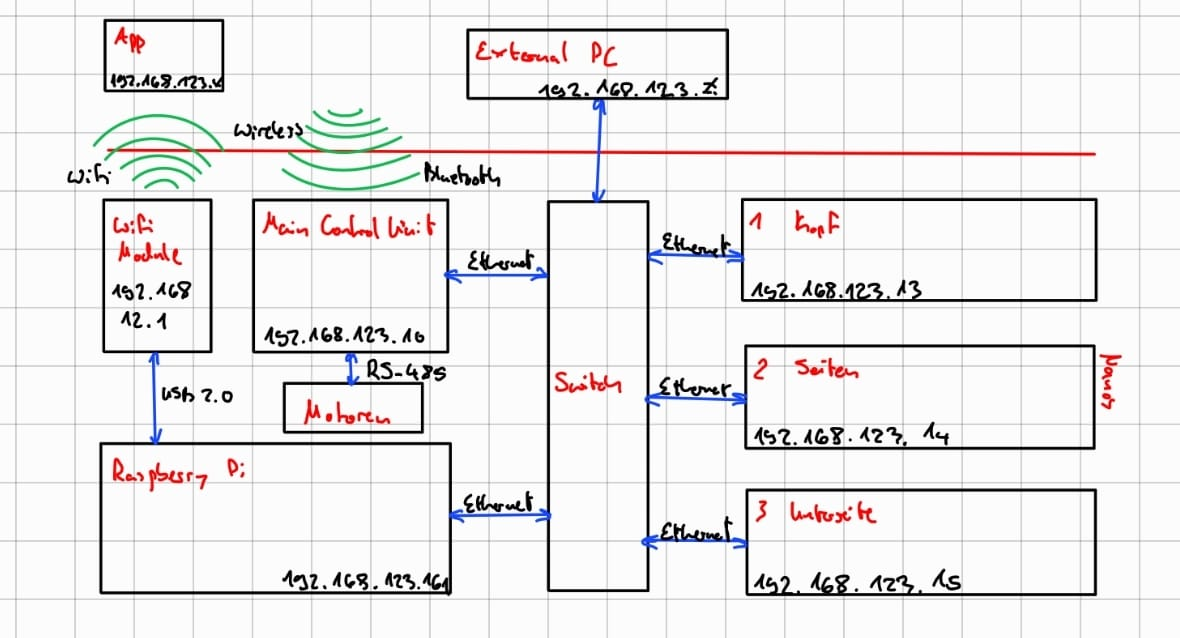
\includegraphics[width=\linewidth]{img/netzwerk/netzwerk_ueberblick}}
    \caption{Überblick über Netzwerkkonfiguration}\label{fig:netzwerk_ueberblick}
\end{figure}\todo{Überblick Quelle aus Anleitung}

Alle geswitchten Komponenten des Netzwerks sind im \texttt{192.168.123.0/24}-Netzwerk registriert.
\todo{was ist gateway? nötig?}
Dabei ist die Verteilung der \gls{ip}-Adressen folgendermaßen vorkonfiguriert:
\begin{itemize}
    \item \textbf{\gls{mcu}:} \texttt{192.168.123.10}
    \item \textbf{Raspberry Pi:} \texttt{192.168.123.10}
    \item \textbf{NVIDIA Jetson Nanos:}
    \begin{enumerate}
        \item Kopf: \texttt{192.168.123.13}
        \item Seiten: \texttt{192.168.123.14}
    \end{enumerate}
    \item \textbf{NVIDIA Jetson Xavier NX:} \texttt{192.168.123.15}
\end{itemize}
Dem Endgerät, das am externen Ethernet-Port an der Oberseite des Roboters angesteckt werden kann,
muss eine statische \gls{ip}-Adresse im Bereich \texttt{192.168.123.0/24} vergeben werden, die nicht bereits von einem der oben genannten
Geräten verwendet wird.

Der Raspberry Pi hat zusätzlich zu seiner physischen Verbindung zum Switch und der \texttt{192.168.123.161}-\gls{ip}-Addresse
noch ein \gls{wwan} Modul verbaut, mit welchem er das Netz \texttt{192.168.12.0/24} publiziert.
Dieses Netz wird ab Werk für die Verbindung der App mit dem System benötigt.
Des Weiteren kann dieses Netz genutzt werden, um eine kabellose Verbindung mit dem Gesamtsystem
des Roboters herzustellen.
Hierzu mehr in Kapitel~\ref{par:raspi}.

\todo{MCU und Bluetooth? Wie?}
\todo{Welche Art Netzwerk, switched, routed, hub?}


